\documentclass[12pt,a4paper]{article}
\usepackage{graphicx}
\usepackage{tabularx}
\usepackage{array}
\usepackage{blindtext}
\usepackage{titlesec}
\usepackage[utf8]{inputenc}
\usepackage{geometry}
\usepackage{ragged2e}
\usepackage{longtable}
\usepackage{listings}
\usepackage{xcolor}
\usepackage{float}
 \geometry{
 a4paper,
 total={170mm,257mm},
 left=19mm,
 top=19mm,
 bottom=19mm,
 right=19mm
 }
\begin{document}
%--------------Title Page ------------------
\thispagestyle{empty}
\begin{center}
\vspace{3cm}
\textbf{\LARGE {Outcome Based Education Management }}\\
\textbf{\LARGE {System }}\\


\vspace{3cm}

\includegraphics[scale=.15]{UETLogo}\\
\vspace{1cm}

Session:2021-2025\\
\vspace{2cm}
\textbf{\large {Submitted by}}\\
\vspace{0.5cm}
\large {Muhammad Hamad Hassan}
\\
\large {2021-CS-33}
\\
\vspace{2cm}
\textbf{\large {Supervised by}}\\
\vspace{0.5cm}
\large {Mr Nauman Babar }
\\

\vspace{3cm}
Department of Computer Science\\
\textbf{\large {University of Engineering and Technology, Lahore}}\\
\textbf{\large {Pakistan}}\\
\end{center}
\newpage
%-----------------Acknowlment------------------
\pagenumbering{roman}
\begin{center}
\textbf{\LARGE {Acknowledgments}}\\
\end{center}
\justifying
I offer my humble gratitude and thanks to the Almighty Allah for His unwavering support and guidance that enabled me to successfully accomplish this endeavor. May His blessings continue to shower upon me in all my future pursuits.

I would like to express my heartfelt gratitude to Mr. Samyan Qayyum Wahla and Mr Nauman Babar for their invaluable guidance, support, and dedication throughout the entire duration of this project. Without their unwavering commitment and expertise, the successful compilation of this project would not have been possible. Their time, effort, and patience have been crucial in ensuring that the project was completed on time and to the highest standard. I am deeply indebted to both of them and feel incredibly privileged to have had the opportunity to work under their guidance.
\newpage

%-----------------Table of Content-----------------------
\tableofcontents
\thispagestyle{empty}
\pagenumbering{arabic}

\newpage




%-----------------List of Figures----------------------
\thispagestyle{empty}
\listoffigures


%-----------------Abstrat-----------------------------
\newpage
\setcounter{page}{1}
\begin{center}
\textbf{\LARGE {Abstract}}\\
\end{center}
\justifying
This report documents the creation of a database system for managing outcome based education using Transact-SQL. The system's design was provided in advance and this report describes the steps taken to develop and implement it. The system contains student data, attendance records, assessment and component records, rubrics and their levels, and CLO details. The report presents a thorough description of the database schema, table relationships, and business rules. It also covers the testing process and challenges faced during development. In summary, this report provides a comprehensive overview of the rubric-based assessment evaluation database system.
\newpage
%-----------------Introduction------------------------
\justifying
\section{Introduction}
\subsection{Description}
Outcome-Based Education (OBE) is a learner-centered educational philosophy that prioritizes the learning outcomes that students should achieve. It aims to align the curriculum with the needs of the industry and society, ensuring that graduates possess the necessary knowledge, skills, and attitudes to excel in their chosen profession. OBE is a holistic approach to education that emphasizes the importance of measurable learning outcomes, as opposed to mere content delivery.

This project is based on the principles of Outcome-Based Education, where a rubric-based assessment evaluation database system was developed to measure and evaluate student learning outcomes. The system manages student data, attendance records, assessment and component records, rubrics and their levels, and CLO details. The database schema, table relationships, and business rules were carefully designed and implemented to align with the principles of OBE.

The system offers a comprehensive approach to evaluating student learning outcomes, enabling educators to assess student progress, identify areas for improvement, and tailor teaching methods to improve student performance. By adopting an OBE philosophy, this project ensures that graduates possess the skills and knowledge required to excel in their chosen profession, aligning with the needs of the industry and society.

In conclusion, this project highlights the importance of Outcome-Based Education in ensuring that graduates possess the necessary skills and knowledge to succeed in their chosen field. The rubric-based assessment evaluation database system developed in this project is an effective tool for measuring and evaluating student learning outcomes and aligns with the principles of OBE.
\subsection{Motivation}
The philosophy of Outcome-Based Education (OBE) prioritizes the learning outcomes that students should achieve, ensuring that graduates possess the necessary skills and knowledge required to excel in their chosen profession. This project highlights the significance of OBE and its relevance to the current education system. By implementing a rubric-based assessment evaluation database system, this project offers an effective approach to evaluating student learning outcomes, enabling educators to tailor teaching methods and identify areas for improvement. The adoption of an OBE philosophy in education is crucial in preparing graduates for the challenges of the modern world, and this project serves as a motivation for educators to embrace this approach to enhance the quality of education and produce competent professionals.
\subsection{Target Audience}
The target audience for this project is educators, curriculum designers, and educational institutions seeking to improve the quality of education and align the curriculum with the needs of the industry and society. The rubric-based assessment evaluation database system developed in this project offers an effective tool for measuring and evaluating student learning outcomes, enabling educators to assess student progress, identify areas for improvement, and tailor teaching methods to enhance student performance. The project's focus on Outcome-Based Education (OBE) philosophy also appeals to curriculum designers and educational institutions looking to adopt a learner-centered approach to education, ensuring that graduates possess the necessary skills and knowledge to succeed in their chosen field. Overall, this project targets individuals and organizations committed to improving the quality of education and preparing graduates for the challenges of the modern world.


%-----------------Operation Detail------------------------
\newpage
\section{Operational Details}
This system is specifically tailored for a solo user, allowing for seamless and efficient management of various academic tasks. With this system, the instructor gains access to a range of features that enable them to manage student data, assessments, assessment components, rubrics, course learning outcomes (CLOs), and student attendance. These features provide a comprehensive approach to academic management, allowing instructors to streamline tasks and improve efficiency. The system is designed to simplify the academic management process, enabling instructors to focus on what matters most - ensuring students receive the best possible education.

%-----------------------Technology Stack----------------

\subsection{Technology Stack}
The system is designed, developed, and tested in a desktop application. The system used the following language, packages, and an Integrated development environment.\\
\begin{longtable}{lr} 
 \caption{Details of technology used in the system. The version number is enclosed in brackets }\\
\begin{tabular}{ | m{4cm} | m{12cm}| } 
  \hline
Language & C \#  (7.3)  \\\hline
IDE  & Microsoft Visual Studio 2022\\ \hline 
Package    &  iTextSharp (5.5.13.3) \\ \hline 
Framework & .Net framework (4.7.2) \\ \hline
UI (user interface) framework    & Windows Presentation Foundation (WPF)\\ \hline
\end{tabular}
\end{longtable}
\subsection{System Requirement}
\begin{longtable}{lr} 
 \caption{To run Outcome Based Education Management  System, your computer must meet the minimum technical specifications outlined below. For optimum performance, use recommended system specifications.}\\
\begin{tabular}{ | m{4cm} | m{12cm}| } \hline
Processor & 
Multicore Intel® or AMD processor (2 GHz or faster processor with SSE 4.2 or later) with 64-bit support
 \\ \hline
Operating system & Windows 8
 \\ \hline
RAM & 4 GB
 \\ \hline
Monitor resolution & 1280 x 800 display at 100%
 \\ \hline
Hard disk space & 1 GB of available hard-disk space
  \\ \hline
\end{tabular}
\end{longtable}
%-----------------Database Design------------------------
\section{Database Design}
Type Here
\begin{figure}[H]
  \centering
    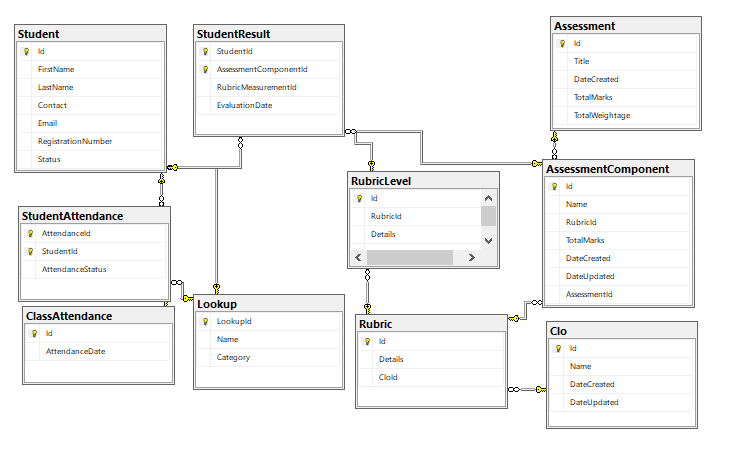
\includegraphics[scale=1]{DatabaseDesign}
  \caption{Database Design}
\end{figure}

\subsection{Student}
The student relation is responsible for storing information related to students, such as their names, contact details, and registration number. The table acts as a central repository for student data, which can be accessed by other tables in the database for various academic management tasks.
\subsection{Lookup}
The lookup relation is utilized to retrieve data from a reference table, where specific values are stored as strings for given foreign keys. The lookup function is used to obtain the scalar equivalent of these foreign keys, facilitating the retrieval of relevant information from the database.
\subsection{Class Attendance}
The class attendance relation is used to record attendance data for each student in a particular date.
\subsection{Student Attendance}
The student attendance relation is used to track and manage student attendance data for each class attendance. 
\subsection{CLO}
CLO stands for Course Learning Outcomes. The CLO relation is used to store information related to the specific learning outcomes that are expected to be achieved by students upon completing a particular course. 
\subsection{Rubric}
Rubrics are used to evaluate student performance against specific criteria related to a particular assignment.
\subsection{Rubric Level}
Rrubric levels are used to define the different levels of performance associated with each criterion in a rubric. 
\subsection{Assessment}
Assessments are used to evaluate student learning and progress towards specific learning outcomes. 
\subsection{Assessment Component}
Assessment questions/component are used to measure specific aspects of student learning related to a particular learning outcome. The assessment question relation stores information related to the specific questions used in an assessment
\subsection{Student Result}
Student results are calculated based on their rubric level, assessment component, and student ID. The system uses this information to generate a comprehensive overview of each student's progress towards achieving specific learning outcomes. 
%-----------------Activity Diagram------------------------
\section{Activity Diagram}
Activity diagrams are a visual representation of the flow of activities and actions within a system. They are commonly used in software development to help illustrate the steps and interactions involved in a particular process or functionality. By mapping out the activities and their relationships, activity diagrams can aid in the design, implementation, and testing phases of software development.
\subsection{Student Management}
\begin{figure}[H]
  \centering
    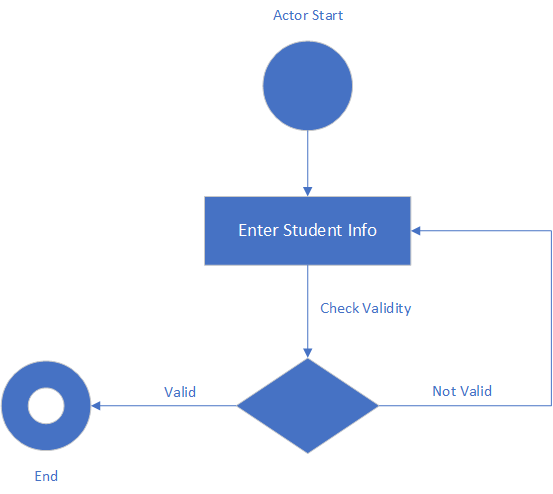
\includegraphics[scale=1]{Student}
    
  \caption{Manage the students}
\end{figure}
\subsection{Attendance Management}
Type Here
\begin{figure}[H]
  \centering
    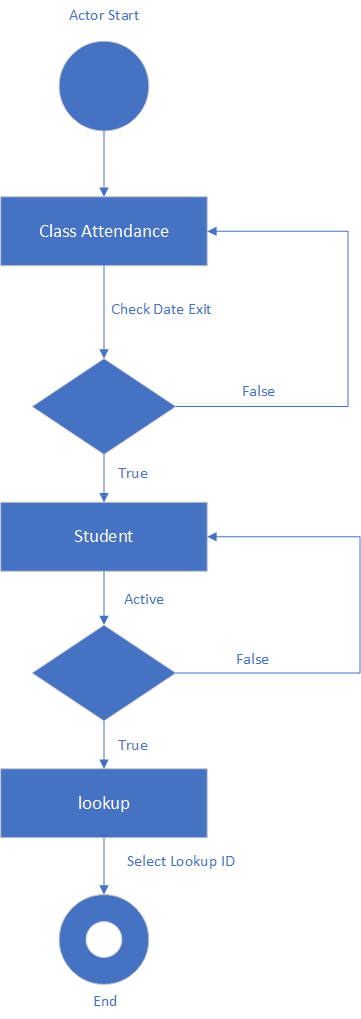
\includegraphics[scale=1]{Student Attendance}

    
  \caption{Manage the attendance}
\end{figure}
\subsection{Assessment Management}
Type Here
\begin{figure}[H]
  \centering
    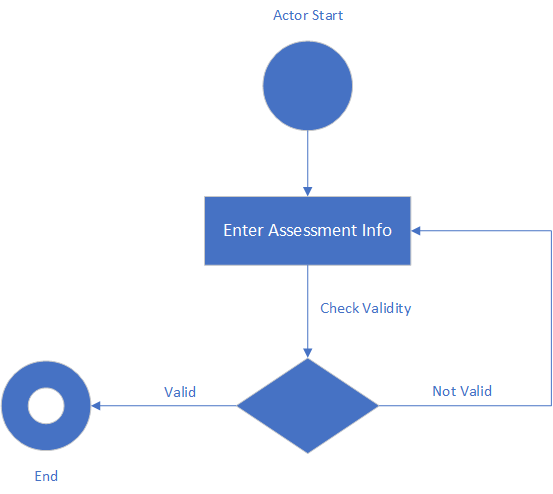
\includegraphics[scale=1]{Assessment}

  \caption{Manage the assessment}
\end{figure}
\subsection{Assessment Component Management}
Type Here
\begin{figure}[H]
  \centering
    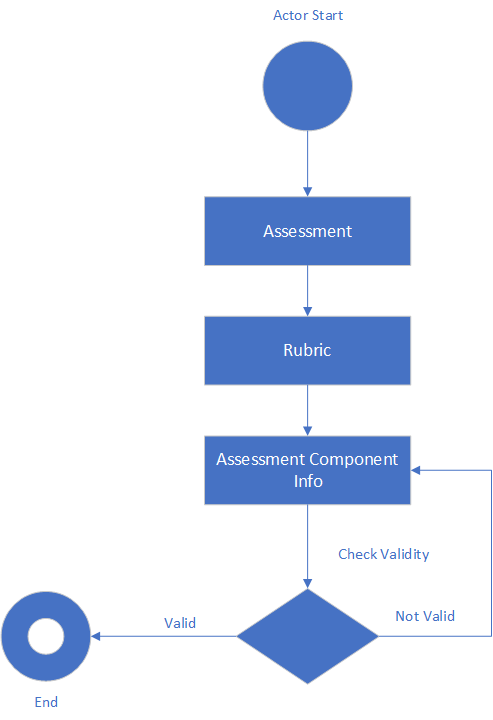
\includegraphics[scale=1]{Assessment Component}

  \caption{Manage the assessment component}
\end{figure}
\subsection{Rubric Management}
Type Here
\begin{figure}[H]
  \centering
    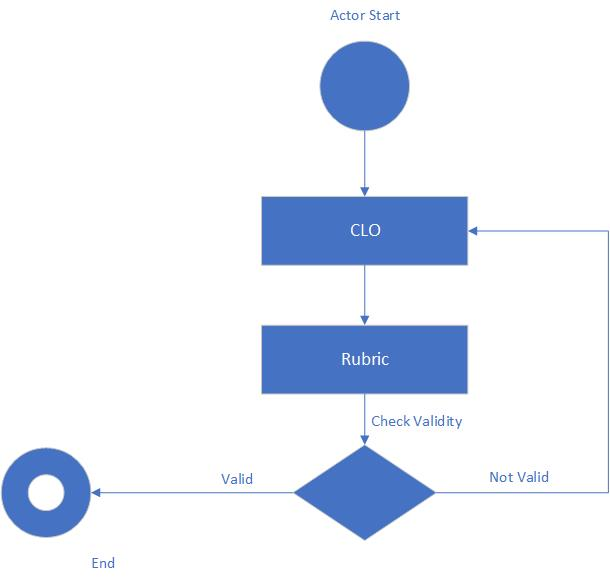
\includegraphics[scale=1]{Rubric}
    
  \caption{Manage the rubric}
\end{figure}
\subsection{Rubric Level Management}
Type Here
\begin{figure}[H]
  \centering
    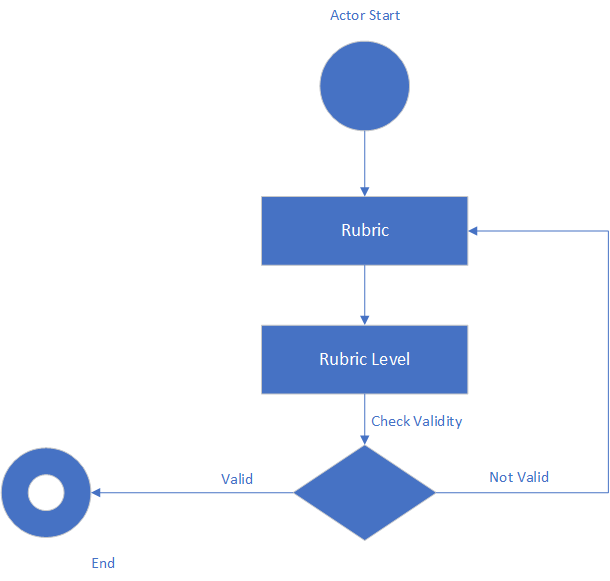
\includegraphics[scale=1]{Rubric Level}
    
  \caption{Manage the rubric level}
\end{figure}
\subsection{CLO Management}
Type Here
\begin{figure}[H]
  \centering
    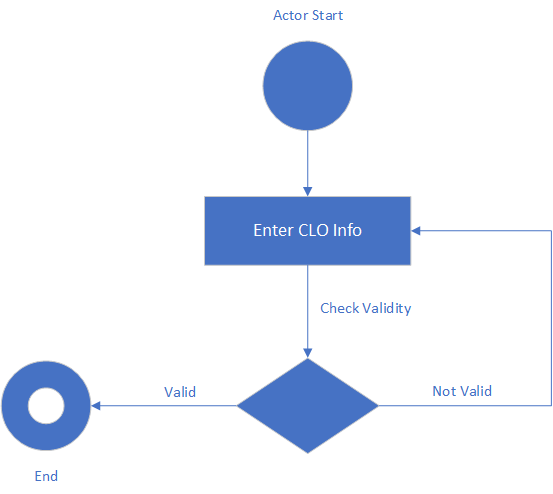
\includegraphics[scale=1]{CLO}
    
  \caption{Manage the clo}
\end{figure}
\subsection{Student Result Management}
Type Here
\begin{figure}[H]
  \centering
    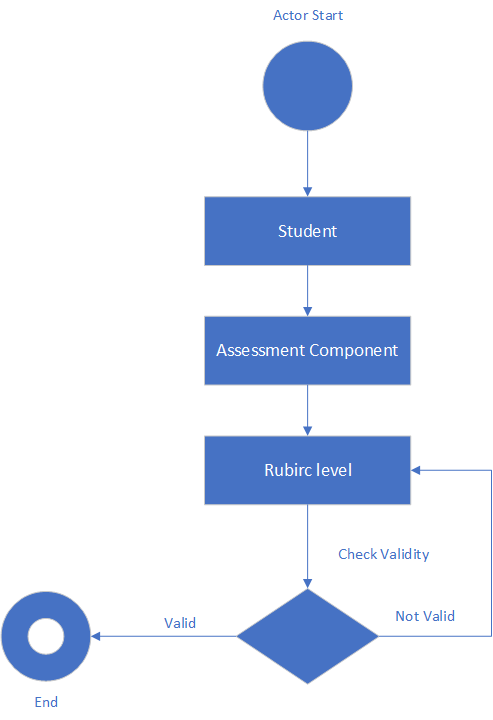
\includegraphics[scale=1]{Student Result}

    
  \caption{Manage the student result}
\end{figure}
%-----------------GUI------------------------

\section{Graphical User Interface}
Type Here
\subsection{Student Management}

\subsubsection{Edit and Delete Student}
\begin{figure}[H]
  \centering
    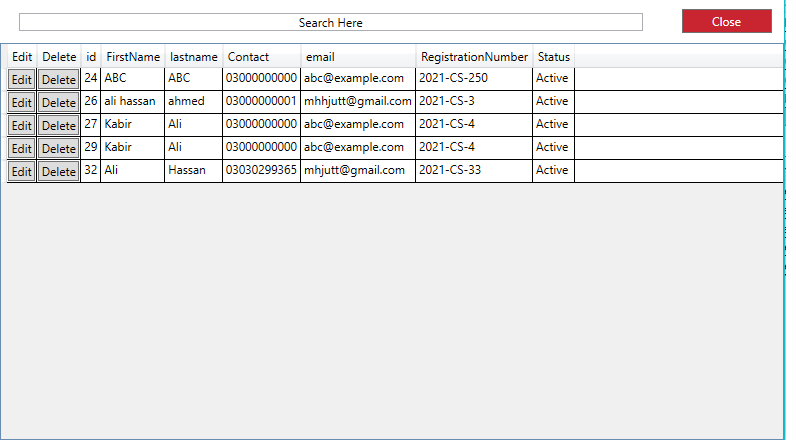
\includegraphics[scale=0.8]{GUIViewStudent}
    
  \caption{Edit and delete the student page}
\end{figure}
\subsubsection{Update and Add Student}
\begin{figure}[H]
  \centering
   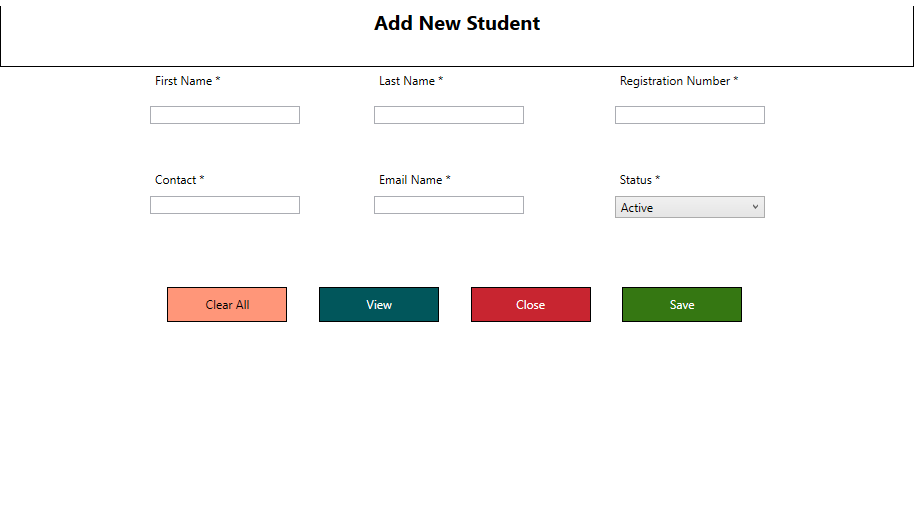
\includegraphics[scale=0.6]{GUIAddStudent}
   
  \caption{Add and update student info page}
\end{figure}


\subsection{Attendance Management}
Type Here
\subsubsection{Mark Attendance}
\begin{figure}[H]
  \centering
  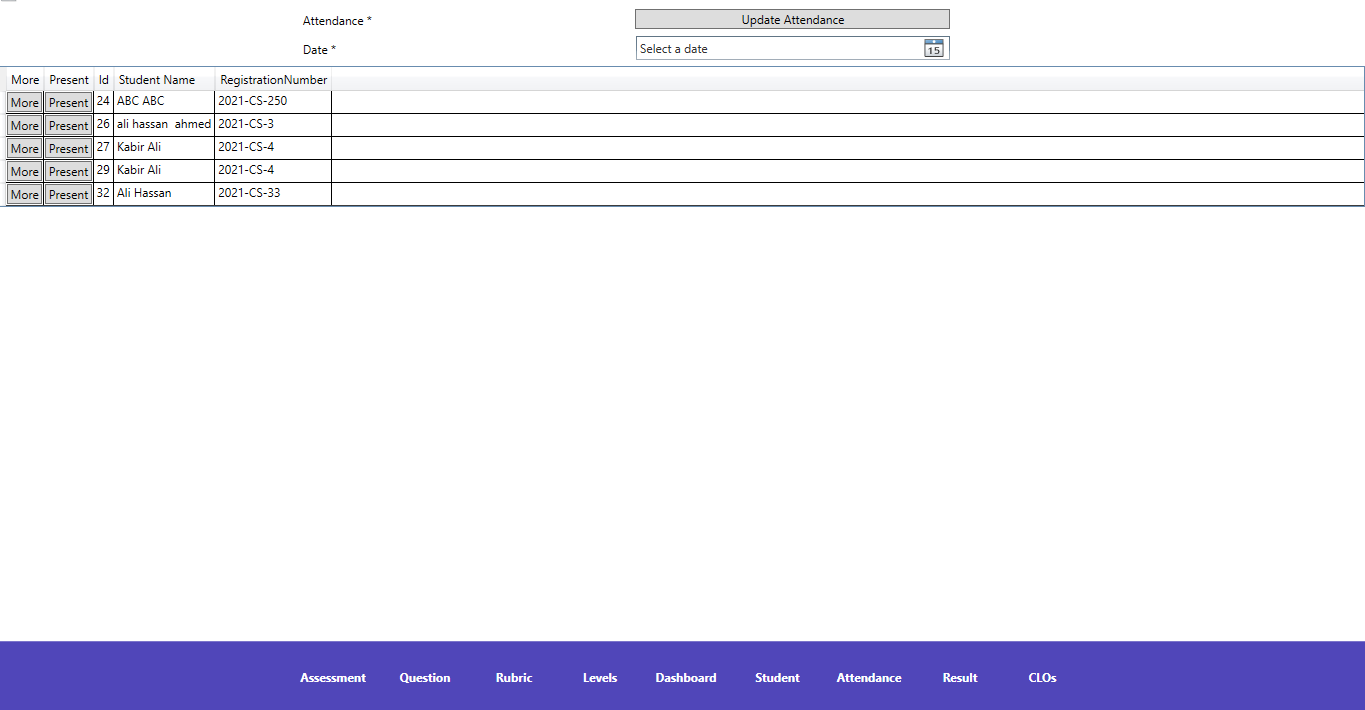
\includegraphics[scale=0.5]{GUIAddAttendance}
  
  \caption{Mark the student attendance page}
\end{figure}


\subsubsection{View Attendance}
\begin{figure}[H]
  \centering
  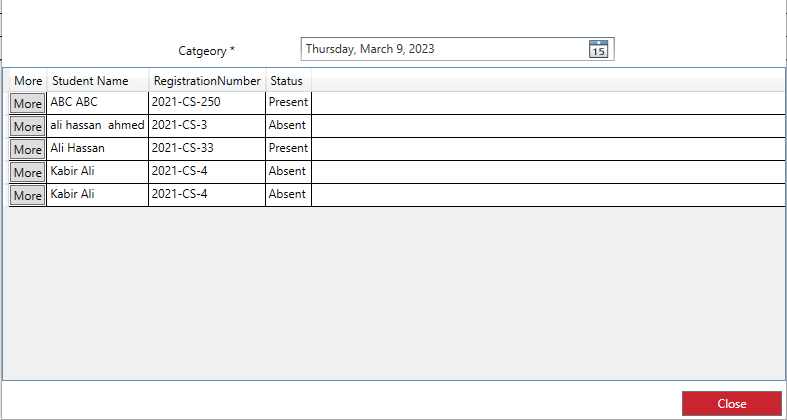
\includegraphics[scale=0.8]{GUIUpdateAttendance}

  \caption{View the mark student attendance page}
\end{figure}


\subsubsection{Update Attendance}

\begin{figure}[H]
  \centering
  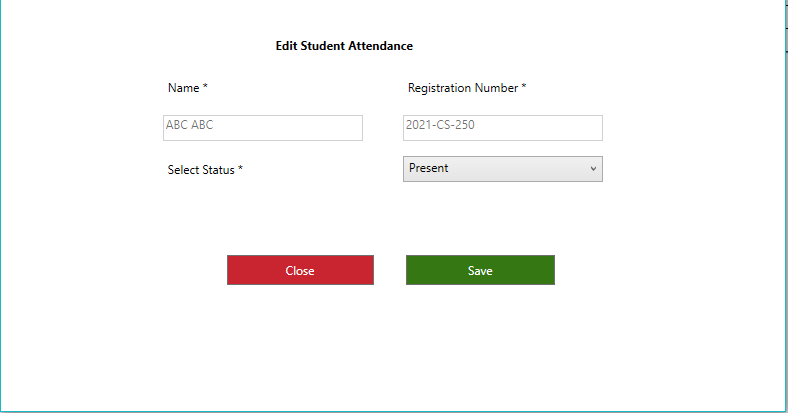
\includegraphics[scale=0.8]{GUIUpdateEditAttendance}

  \caption{Update the mark student attendance page}
\end{figure}


\subsection{Assessment Management}
Type Here

\begin{figure}[H]
  \centering
  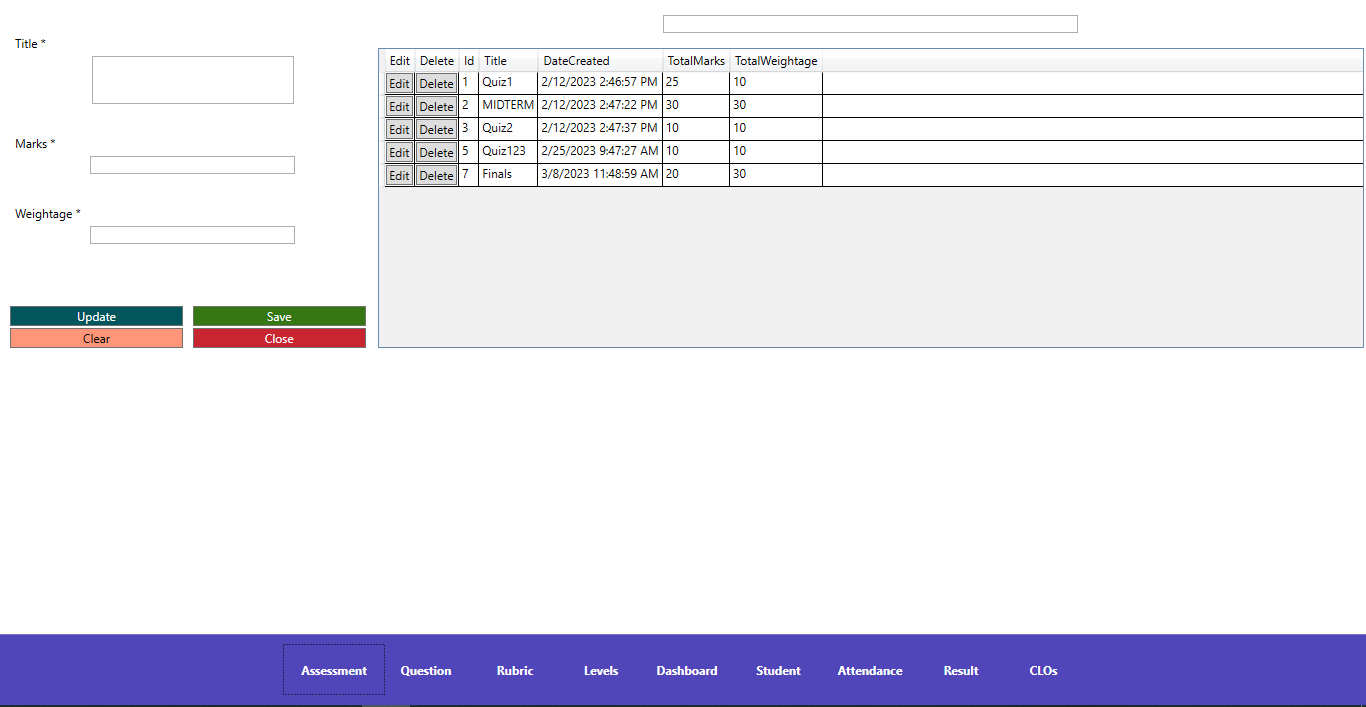
\includegraphics[scale=0.5]{GUIAssessment}

  \caption{View, create, update and delete the assessment page}
\end{figure}

\subsection{Assessment Component Management}
Type Here

\begin{figure}[H]
  \centering
  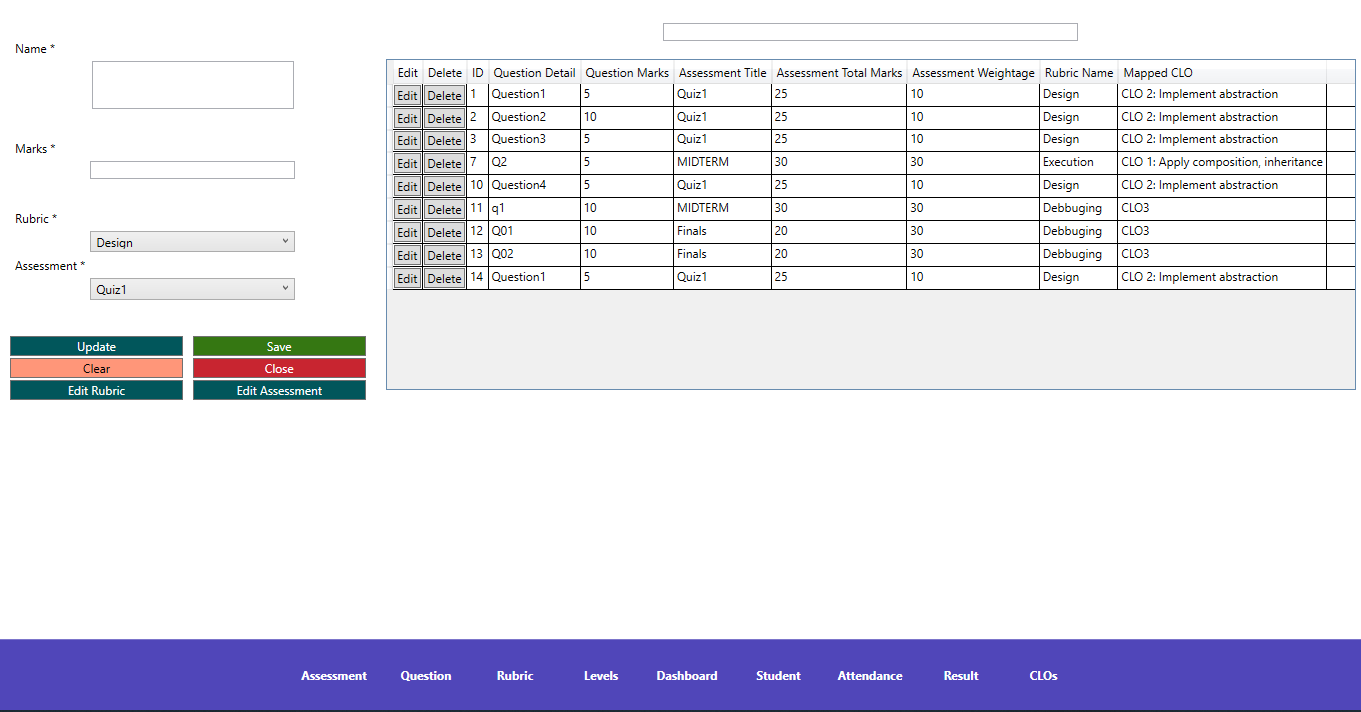
\includegraphics[scale=0.5]{GUIAssessmentComponent}

  \caption{View, create, update and delete the assessment component page}
\end{figure}

\subsection{Rubric Management}
Type Here

\begin{figure}[H]
  \centering
  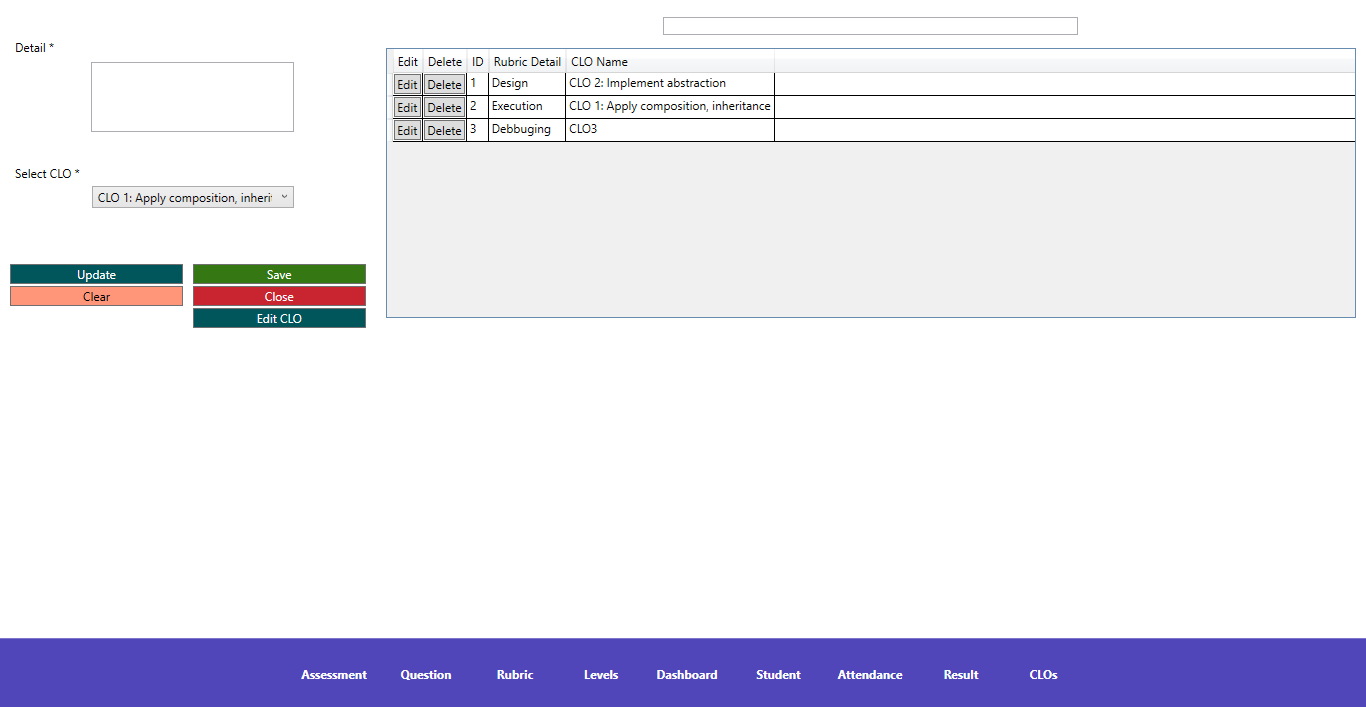
\includegraphics[scale=0.5]{GUIRubric}

  \caption{View, create, update and delete the rubric page}
\end{figure}

\subsection{Rubric Level Management}
Type Here

\begin{figure}[H]
  \centering
  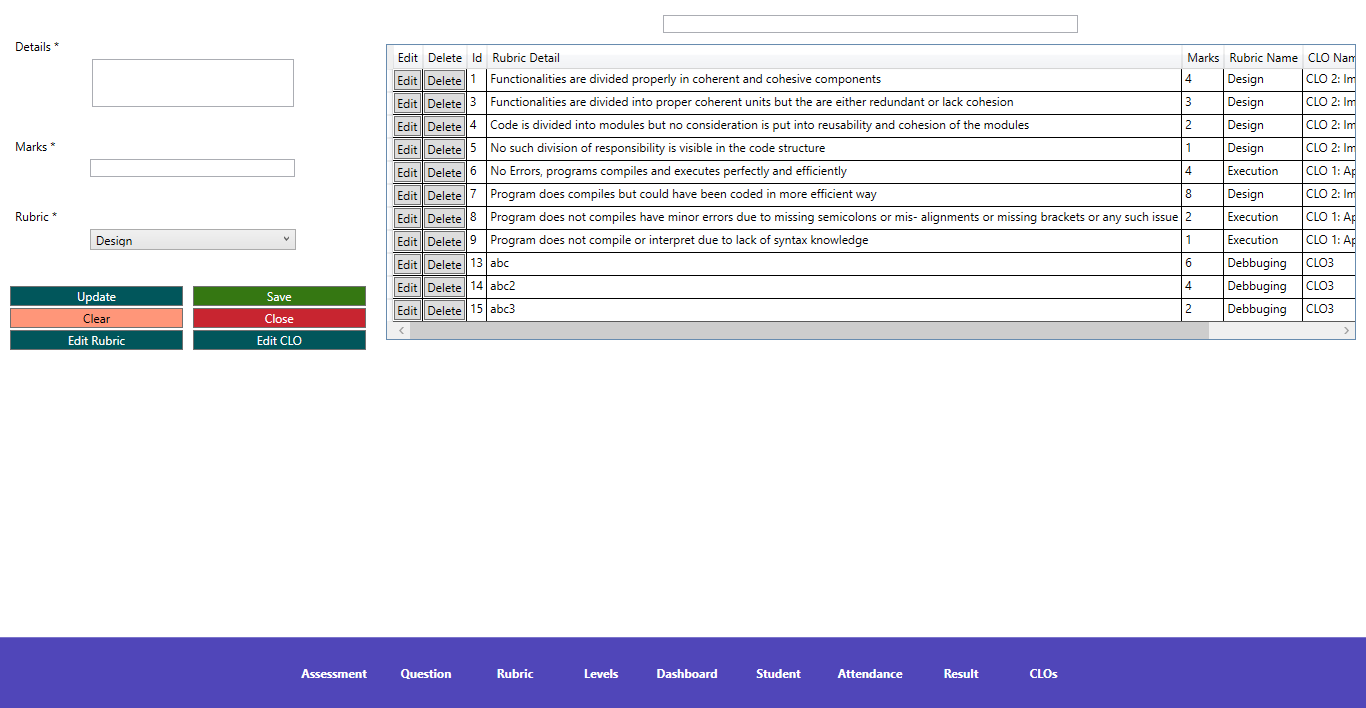
\includegraphics[scale=0.5]{GUIRubricLevel}

  \caption{View, create, update and delete the rubric level page}
\end{figure}

\subsection{CLO Management}
Type Here

\begin{figure}[H]
  \centering
  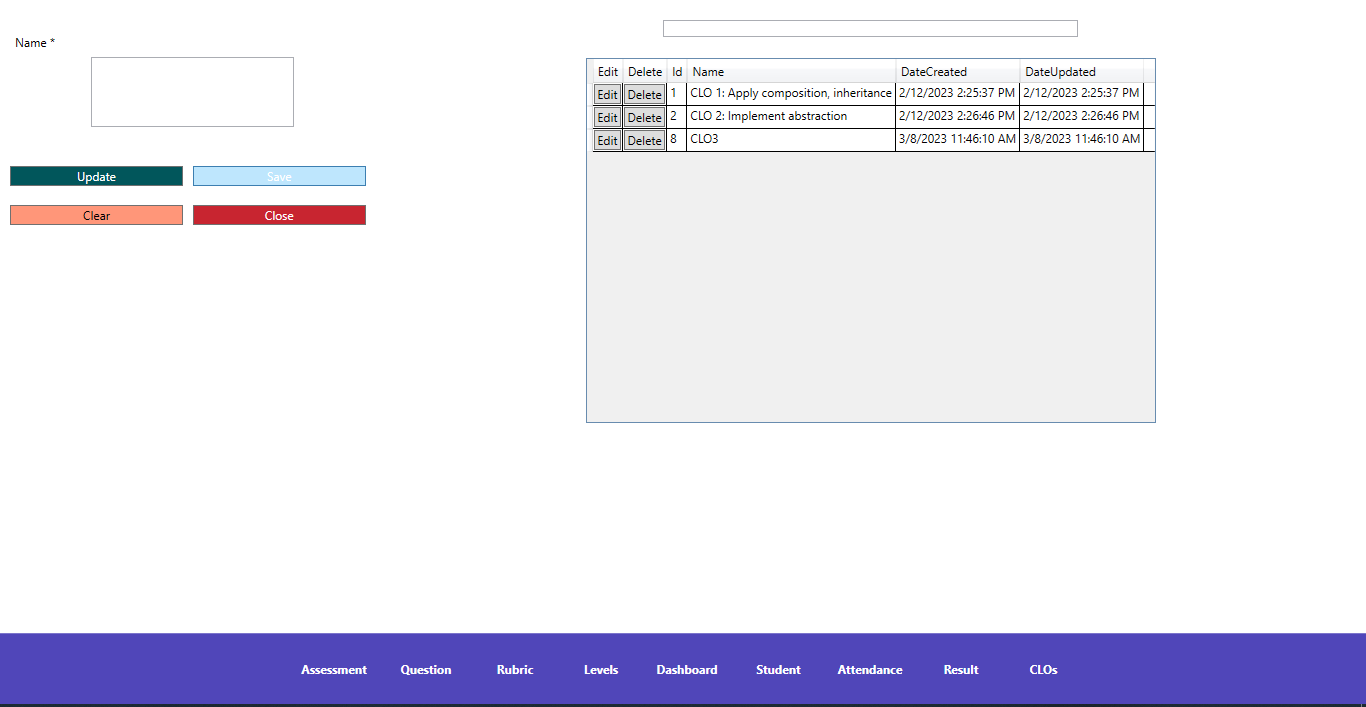
\includegraphics[scale=0.5]{GUICLO}

  \caption{View, create, update and delete the clo page}
\end{figure}

\subsection{Student Result Management}
Type Here
\begin{figure}[H]
  \centering
  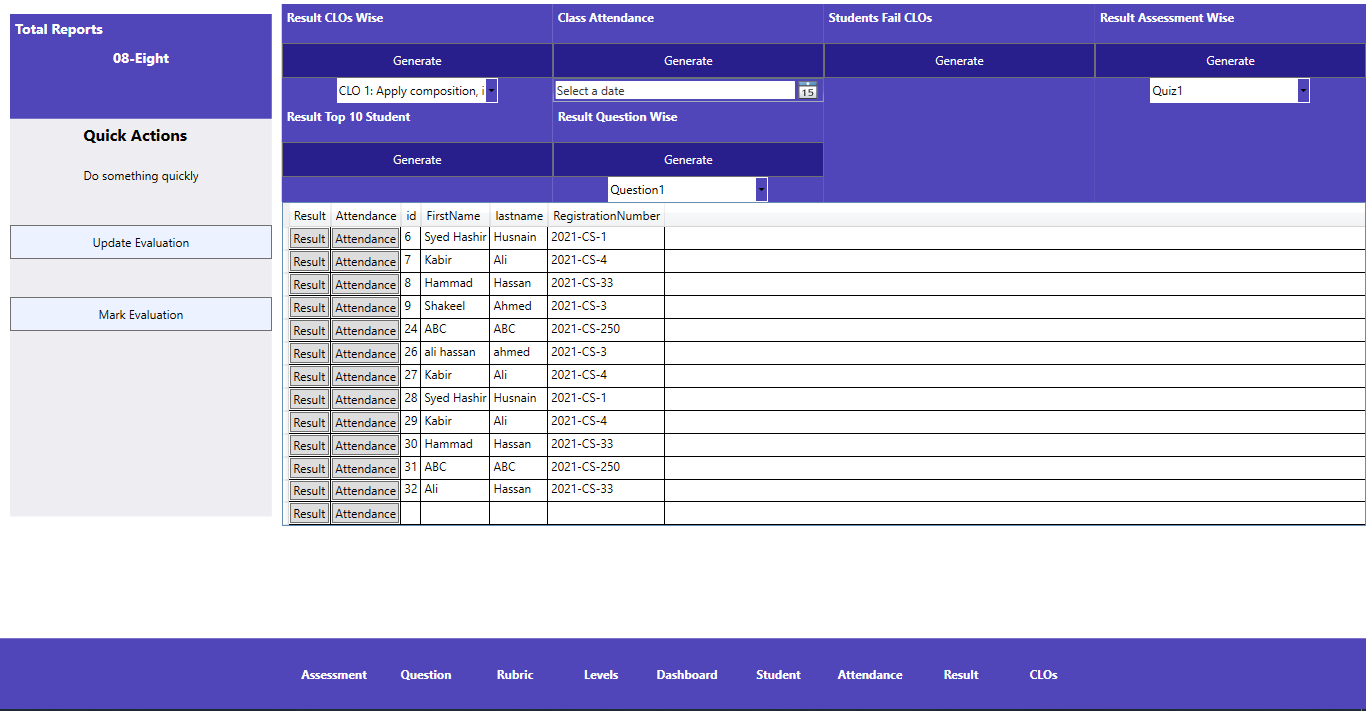
\includegraphics[scale=0.5]{GUIResult}

  \caption{View and mark the evaluation and generate different reports page}
\end{figure}

%------------------SET SQL Environment-----------
\lstnewenvironment{sql}[1][]
{\lstset{language=SQL,basicstyle=\ttfamily,#1,xleftmargin=0.5cm,xrightmargin=0.5cm}}{}
% Define a custom style for SQL listings
\lstdefinestyle{sqlStyle}{
  language=SQL,
  basicstyle=\ttfamily,
  keywordstyle=\color{blue}\bfseries,
  keywords={SELECT,FROM,WHERE}
}

%-----------------Generated Reports------------------------
\section{Generated Reports}
Type Here
\subsection{Result CLO Wise}
\begin{sql}[style=sqlStyle]
SELECT CONCAT(Max(S.FirstName),' ',Max(S.LastName))AS [StudentName],
S.RegistrationNumber,
A.Title AS Assignment,A.TotalMarks,SUM((CAST (RL.MeasurementLevel
 AS float)/ML.MaxLevel)*AC.TotalMarks) AS [ObtainedMarks],
C.Name AS [CLOName]
FROM Student S
JOIN StudentResult SR
ON SR.StudentId=S.Id
JOIN AssessmentComponent AC
ON AC.Id=SR.AssessmentComponentId
JOIN RubricLevel RL
ON RL.Id=SR.RubricMeasurementId
JOIN  Assessment A
ON A.Id=AC.AssessmentId
JOIN (SELECT RL1.RubricId,MAX(RL1.MeasurementLevel) AS MaxLevel 
FROM RubricLevel RL1 GROUP BY RubricId) AS ML
ON ML.RubricId=AC.RubricId
JOIN Rubric R
ON R.Id=AC.RubricId
JOIN Clo C
ON C.Id=R.CloId
WHERE C.Id=2
GROUP BY S.RegistrationNumber,A.Title,A.TotalMarks,C.Name
ORDER BY C.Name ASC;
\end{sql}

\subsection{Class Attendance}
\begin{sql}[style=sqlStyle]
SELECT CONCAT(S.FirstName,' ',S.LastName)AS Name,
S.RegistrationNumber,L.Name
FROM Student S
JOIN StudentAttendance ST
ON S.Id=ST.StudentId
JOIN ClassAttendance C
ON C.Id=ST.AttendanceId
JOIN Lookup L
ON L.LookupId=ST.AttendanceStatus
WHERE L.Category='ATTENDANCE_STATUS'
 AND C.AttendanceDate='2023-03-10 00:00:00.000'
\end{sql}
\subsection{Student Fail CLO}
\begin{sql}[style=sqlStyle]
SELECT CONCAT(Max(S.FirstName),' ',Max(S.LastName))AS [StudentName],
S.RegistrationNumber,A.Title AS Assignment,A.TotalMarks,
SUM((CAST (RL.MeasurementLevel AS float)/ML.MaxLevel)
*AC.TotalMarks) AS [ObtainedMarks],
C.Name AS [CLOName]
FROM Student S
JOIN StudentResult SR
ON SR.StudentId=S.Id
JOIN AssessmentComponent AC
ON AC.Id=SR.AssessmentComponentId
JOIN RubricLevel RL
ON RL.Id=SR.RubricMeasurementId
JOIN  Assessment A
ON A.Id=AC.AssessmentId
JOIN (SELECT RL1.RubricId,MAX(RL1.MeasurementLevel) AS MaxLevel
FROM RubricLevel RL1 GROUP BY RubricId) AS ML
ON ML.RubricId=AC.RubricId
JOIN Rubric R
ON R.Id=AC.RubricId
JOIN Clo C
ON C.Id=R.CloId
GROUP BY S.RegistrationNumber,A.Title,A.TotalMarks,C.Name
HAVING  ((SUM((CAST (RL.MeasurementLevel AS float)/ML.MaxLevel)*
AC.TotalMarks))/A.TotalMarks)*100<=33
ORDER BY C.Name ASC
\end{sql}
\subsection{Result Asssessment Wise}
\begin{sql}[style=sqlStyle]
SELECT CONCAT(Max(S.FirstName),' ',Max(S.LastName))AS [StudentName],
S.RegistrationNumber,A.Title AS Assignment,A.TotalMarks,
SUM((CAST (RL.MeasurementLevel AS float)/ML.MaxLevel)*AC.TotalMarks) 
AS [ObtainedMarks]
FROM Student S
JOIN StudentResult SR
ON SR.StudentId=S.Id
JOIN AssessmentComponent AC
ON AC.Id=SR.AssessmentComponentId
JOIN RubricLevel RL
ON RL.Id=SR.RubricMeasurementId
JOIN  Assessment A
ON A.Id=AC.AssessmentId
JOIN (SELECT RL1.RubricId,MAX(RL1.MeasurementLevel) AS MaxLevel 
FROM RubricLevel RL1 GROUP BY RubricId) AS ML
ON ML.RubricId=AC.RubricId
JOIN Rubric R
ON R.Id=AC.RubricId
JOIN Clo C
ON C.Id=R.CloId
WHERE A.Id=2
GROUP BY S.RegistrationNumber,A.Title,A.TotalMarks
ORDER BY  A.Title ASC
\end{sql}
\subsection{Result Top 10 Student}
\begin{sql}[style=sqlStyle]
SELECT TOP 10 CONCAT(Max(S.FirstName),' ',Max(S.LastName))
AS [StudentName],
S.RegistrationNumber,A.Title AS Assignment,A.TotalMarks,
SUM((CAST (RL.MeasurementLevel AS float)/ML.MaxLevel)*
AC.TotalMarks) AS [Obtained Marks]
FROM Student S
JOIN StudentResult SR
ON SR.StudentId=S.Id
JOIN AssessmentComponent AC
ON AC.Id=SR.AssessmentComponentId
JOIN RubricLevel RL
ON RL.Id=SR.RubricMeasurementId
JOIN  Assessment A
ON A.Id=AC.AssessmentId
JOIN (SELECT RL1.RubricId,MAX(RL1.MeasurementLevel) AS MaxLevel 
FROM RubricLevel RL1 GROUP BY RubricId) AS ML
ON ML.RubricId
=AC.RubricId
GROUP BY S.RegistrationNumber,A.Title,A.TotalMarks
ORDER BY [Obtained Marks] DESC
\end{sql}
\subsection{Result Question Wise}
\begin{sql}[style=sqlStyle]
SELECT CONCAT(Max(S.FirstName),' ',Max(S.LastName))AS [StudentName],
S.RegistrationNumber,A.Title AS Assignment,AC.TotalMarks,
SUM((CAST (RL.MeasurementLevel AS float)/ML.MaxLevel)*
AC.TotalMarks) AS [ObtainedMarks]
,AC.Name AS QuestionName
FROM Student S
JOIN StudentResult SR
ON SR.StudentId=S.Id
JOIN AssessmentComponent AC
ON AC.Id=SR.AssessmentComponentId
JOIN RubricLevel RL
ON RL.Id=SR.RubricMeasurementId
JOIN  Assessment A
ON A.Id=AC.AssessmentId
JOIN (SELECT RL1.RubricId,MAX(RL1.MeasurementLevel) AS MaxLevel FROM
 RubricLevel RL1 GROUP BY RubricId) AS ML
ON ML.RubricId
=AC.RubricId
JOIN Rubric R
ON R.Id=AC.RubricId
JOIN Clo C
ON C.Id=R.CloId
WHERE AC.Id=2
GROUP BY S.RegistrationNumber,A.Title,AC.TotalMarks,AC.Name
ORDER BY  AC.Name ASC
\end{sql}
\subsection{Specfic Student Result }
\begin{sql}[style=sqlStyle]
SELECT CONCAT(Max(S.FirstName),' ',Max(S.LastName))AS [StudentName],
A.Title AS Assignment,SUM((CAST (RL.MeasurementLevel
AS float)/ML.MaxLevel)
*AC.TotalMarks) AS [Obtained Marks],A.TotalMarks
FROM Student S
JOIN StudentResult SR
ON SR.StudentId=S.Id
JOIN AssessmentComponent AC
ON AC.Id=SR.AssessmentComponentId
JOIN RubricLevel RL
ON RL.Id=SR.RubricMeasurementId
JOIN  Assessment A
ON A.Id=AC.AssessmentId
JOIN (SELECT RL1.RubricId,MAX(RL1.MeasurementLevel) AS MaxLevel 
FROM RubricLevel RL1 GROUP BY RubricId) AS ML
ON ML.RubricId=
AC.RubricId
WHERE S.Id=24
GROUP BY S.RegistrationNumber,A.Title,A.TotalMarks
ORDER BY S.RegistrationNumber ASC
\end{sql}
\subsection{Specfic Student Attendance }
\begin{sql}[style=sqlStyle]
SELECT  CONVERT(date,  C.AttendanceDate, 101) AS Date ,L.Name
FROM Student S
JOIN StudentAttendance ST
ON S.Id=ST.StudentId
JOIN ClassAttendance C
ON C.Id=ST.AttendanceId
JOIN Lookup L
ON L.LookupId=ST.AttendanceStatus
WHERE S.Id=29
ORDER BY DATE DESC
\end{sql}
%-----------------Testing------------------------
\section{Testing}
Throughout my development process, I conducted testing at every stage with each commit, ensuring that any bugs were identified and addressed before they became significant issues. This approach allowed me to tackle and resolve minor issues, preventing them from snowballing into major problems.

During the testing phase of the Outcome Based Education Management System application, the primary challenge was the lack of a specific format for generating PDF reports. However, I made every effort to create reports that were clear and readable for instructors, despite the absence of a prescribed format. The rigorous testing process I employed during development ensured that the  Outcome Based Education Management System application was robust and reliable, providing instructors with accurate and useful information to support student success.

%-----------------Limitations------------------------
\section{Limitations}
One of the limitations of the system is that it is designed for a single class, single course scenario, and cannot be easily scaled to accommodate multiple classes or courses. Additionally, the system's user interface is currently limited to desktop platforms and does not support mobile devices. The system's reporting functionality is also limited to generating PDF reports without any formatting options. These limitations may restrict the system's usage in certain scenarios and may require additional development efforts to address them.
%-----------------Future Work------------------------
\section{Future Work}
To address the limitations of the current system, future development efforts will focus on implementing a more scalable architecture based on the principles of Object-Oriented Programming (OOP). This will involve separating the system into distinct layers, including a User Interface (UI) layer, Business Logic (BL) layer, and Data Access Layer (DAL). Additionally, efforts will be made to enhance the system's reporting functionality by introducing formatting options for the generated PDF reports. Finally, the system will be optimized for use on mobile devices to provide greater flexibility in accessing and using the system. These improvements will allow the system to be used in a wider range of scenarios and provide a more user-friendly experience for instructors and students alike.
%-----------------Collaboration------------------------
\section{Collaboration}
The successful completion of this project was made possible thanks to the invaluable guidance of our supervisors, Mr. Nouman Babar and Mr. Samyan Wahla, as well as the support of my friends who were always available to discuss and troubleshoot any conceptual issues.

%-----------------Conclusion------------------------
\section{Conclusion}
The design and implementation of the rubric-based assessment evaluation system has been successfully accomplished. The project has demonstrated the use of Outcome-Based Education in the development of a database system. The system provides a user-friendly interface to manage student data, attendance records, assessment and assessment component records, rubrics and their levels, and CLO details. The testing and debugging phase ensured that the system is free of errors and meets the requirements specified in the project brief. The limitations of the system were also discussed, and future work was proposed to improve the system's functionality. The successful completion of this project would not have been possible without the guidance of our supervisors and the support of our colleagues, and it has provided valuable insights into database management systems and their applications in education sector.





\end{document}